\section{Engine\-Subject Class Reference}
\label{classEngineSubject}\index{EngineSubject@{EngineSubject}}
{\tt \#include $<$engineobserver.h$>$}

Inheritance diagram for Engine\-Subject:\begin{figure}[H]
\begin{center}
\leavevmode
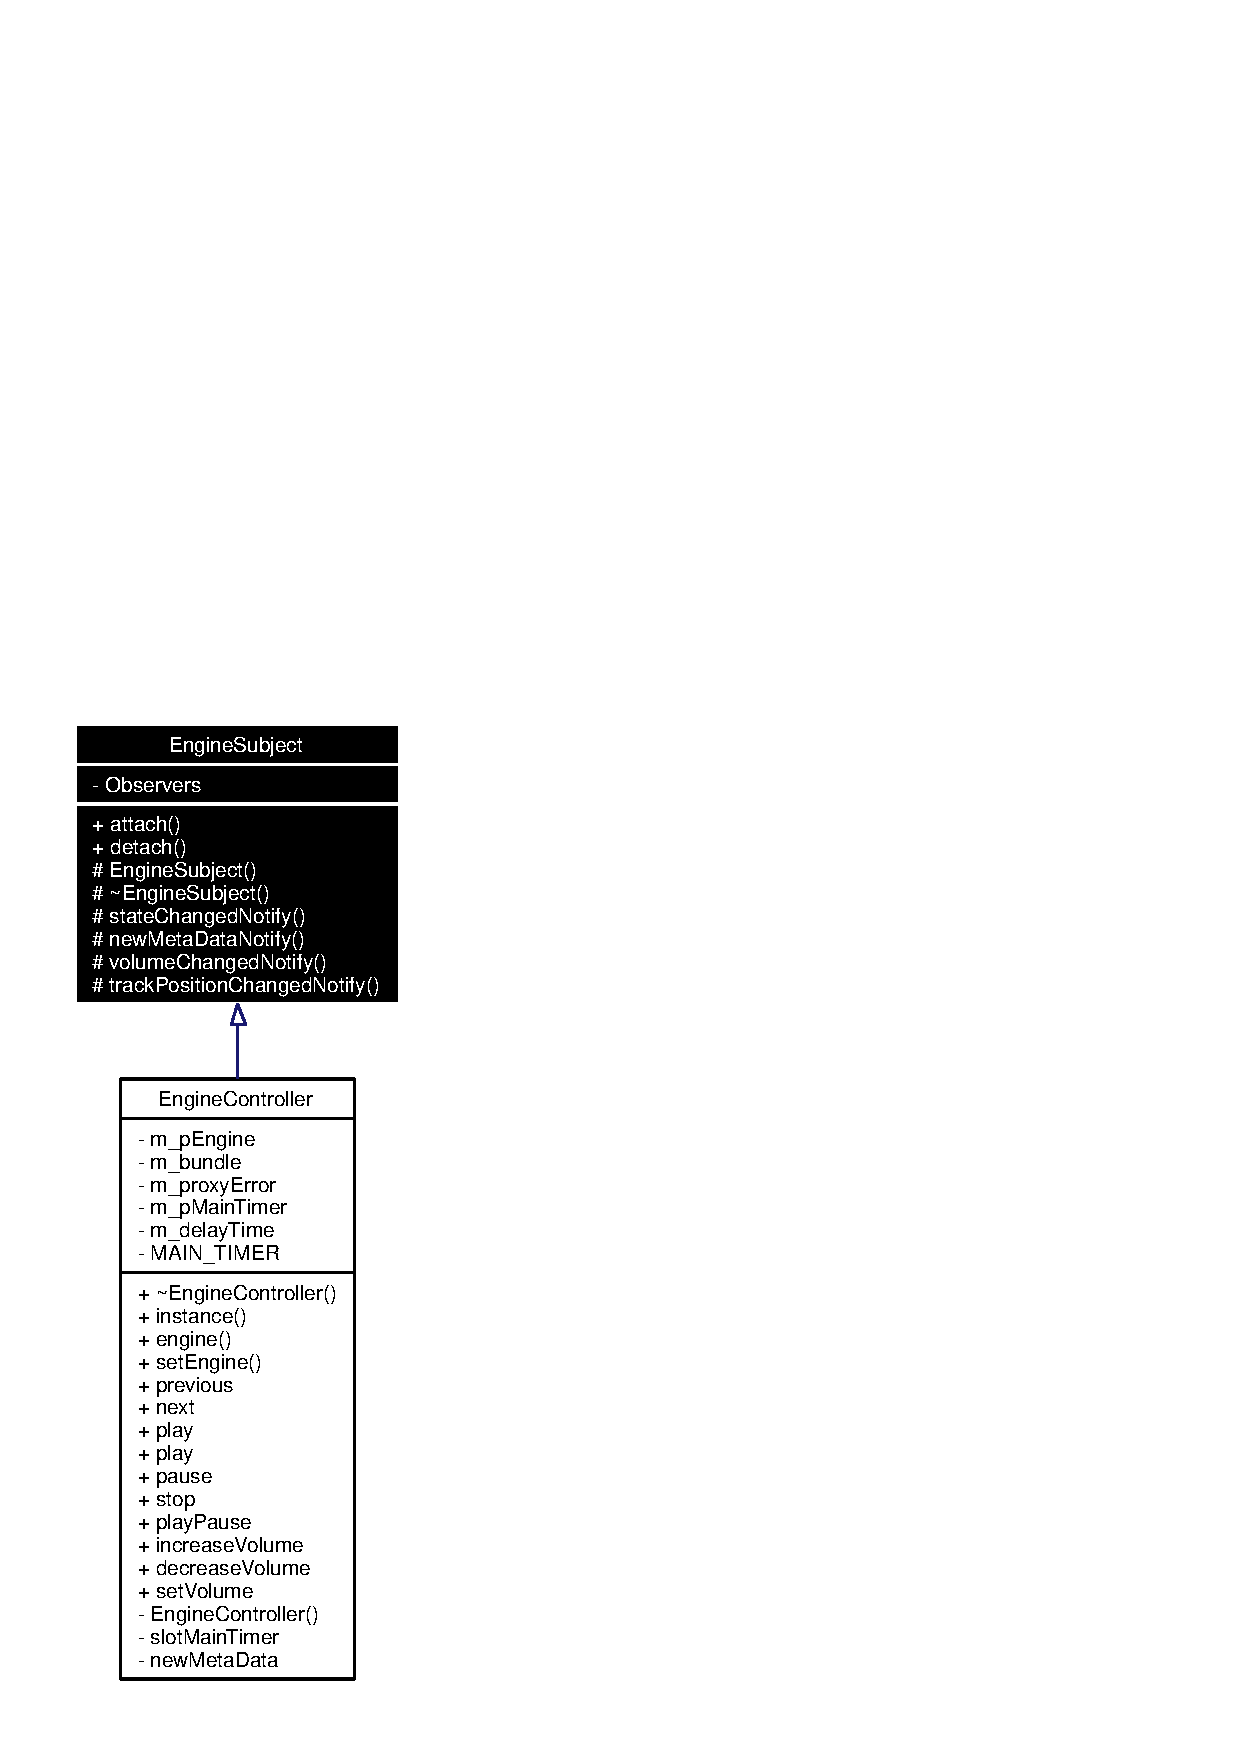
\includegraphics[width=96pt]{classEngineSubject__inherit__graph}
\end{center}
\end{figure}


\subsection{Detailed Description}
Inherited by {\bf Engine\-Controller}{\rm (p.\,\pageref{classEngineController})}. Notify observer functionality is captured in this class. 



Definition at line 45 of file engineobserver.h.\subsection*{Public Member Functions}
\begin{CompactItemize}
\item 
void {\bf attach} ({\bf Engine\-Observer} $\ast$observer)
\item 
void {\bf detach} ({\bf Engine\-Observer} $\ast$observer)
\end{CompactItemize}
\subsection*{Protected Member Functions}
\begin{CompactItemize}
\item 
{\bf Engine\-Subject} ()
\item 
virtual {\bf $\sim$Engine\-Subject} ()
\item 
void {\bf state\-Changed\-Notify} ({\bf Engine\-Base::Engine\-State})
\item 
void {\bf new\-Meta\-Data\-Notify} (const {\bf Meta\-Bundle} \&, bool)
\item 
void {\bf volume\-Changed\-Notify} (int)
\item 
void {\bf track\-Position\-Changed\-Notify} (long)
\end{CompactItemize}
\subsection*{Private Attributes}
\begin{CompactItemize}
\item 
QPtr\-List$<$ {\bf Engine\-Observer} $>$ {\bf Observers}
\end{CompactItemize}


\subsection{Constructor \& Destructor Documentation}
\index{EngineSubject@{Engine\-Subject}!EngineSubject@{EngineSubject}}
\index{EngineSubject@{EngineSubject}!EngineSubject@{Engine\-Subject}}
\subsubsection{\setlength{\rightskip}{0pt plus 5cm}Engine\-Subject::Engine\-Subject ()\hspace{0.3cm}{\tt  [protected]}}\label{classEngineSubject_EngineSubjectb0}




Definition at line 34 of file engineobserver.cpp.



\footnotesize\begin{verbatim}35 {
36 }
\end{verbatim}\normalsize 
\index{EngineSubject@{Engine\-Subject}!~EngineSubject@{$\sim$EngineSubject}}
\index{~EngineSubject@{$\sim$EngineSubject}!EngineSubject@{Engine\-Subject}}
\subsubsection{\setlength{\rightskip}{0pt plus 5cm}Engine\-Subject::$\sim${\bf Engine\-Subject} ()\hspace{0.3cm}{\tt  [protected, virtual]}}\label{classEngineSubject_EngineSubjectb1}




Definition at line 39 of file engineobserver.cpp.



\footnotesize\begin{verbatim}40 {
41 }
\end{verbatim}\normalsize 


\subsection{Member Function Documentation}
\index{EngineSubject@{Engine\-Subject}!attach@{attach}}
\index{attach@{attach}!EngineSubject@{Engine\-Subject}}
\subsubsection{\setlength{\rightskip}{0pt plus 5cm}void Engine\-Subject::attach ({\bf Engine\-Observer} $\ast$ {\em observer})}\label{classEngineSubject_EngineSubjecta0}




Definition at line 92 of file engineobserver.cpp.

References Observers.



\footnotesize\begin{verbatim}93 {
94     if( !observer || Observers.find( observer ) != -1 )
95         return;
96     Observers.append( observer );
97 }
\end{verbatim}\normalsize 
\index{EngineSubject@{Engine\-Subject}!detach@{detach}}
\index{detach@{detach}!EngineSubject@{Engine\-Subject}}
\subsubsection{\setlength{\rightskip}{0pt plus 5cm}void Engine\-Subject::detach ({\bf Engine\-Observer} $\ast$ {\em observer})}\label{classEngineSubject_EngineSubjecta1}




Definition at line 100 of file engineobserver.cpp.

References Observers.



\footnotesize\begin{verbatim}101 {
102     if( Observers.find( observer ) != -1 ) Observers.remove();
103 }
\end{verbatim}\normalsize 
\index{EngineSubject@{Engine\-Subject}!newMetaDataNotify@{newMetaDataNotify}}
\index{newMetaDataNotify@{newMetaDataNotify}!EngineSubject@{Engine\-Subject}}
\subsubsection{\setlength{\rightskip}{0pt plus 5cm}void Engine\-Subject::new\-Meta\-Data\-Notify (const {\bf Meta\-Bundle} \&, bool)\hspace{0.3cm}{\tt  [protected]}}\label{classEngineSubject_EngineSubjectb3}




Definition at line 56 of file engineobserver.cpp.

References Engine\-Observer::engine\-New\-Meta\-Data(), and Observers.

Referenced by Engine\-Controller::play().



\footnotesize\begin{verbatim}57 {
58     QPtrListIterator<EngineObserver> it( Observers );
59     EngineObserver *observer;
60     while( ( observer = it.current() ) != 0 )
61     {
62         ++it;
63         observer->engineNewMetaData( bundle, trackChanged );
64     }
65 }
\end{verbatim}\normalsize 


Here is the call graph for this function:\begin{figure}[H]
\begin{center}
\leavevmode
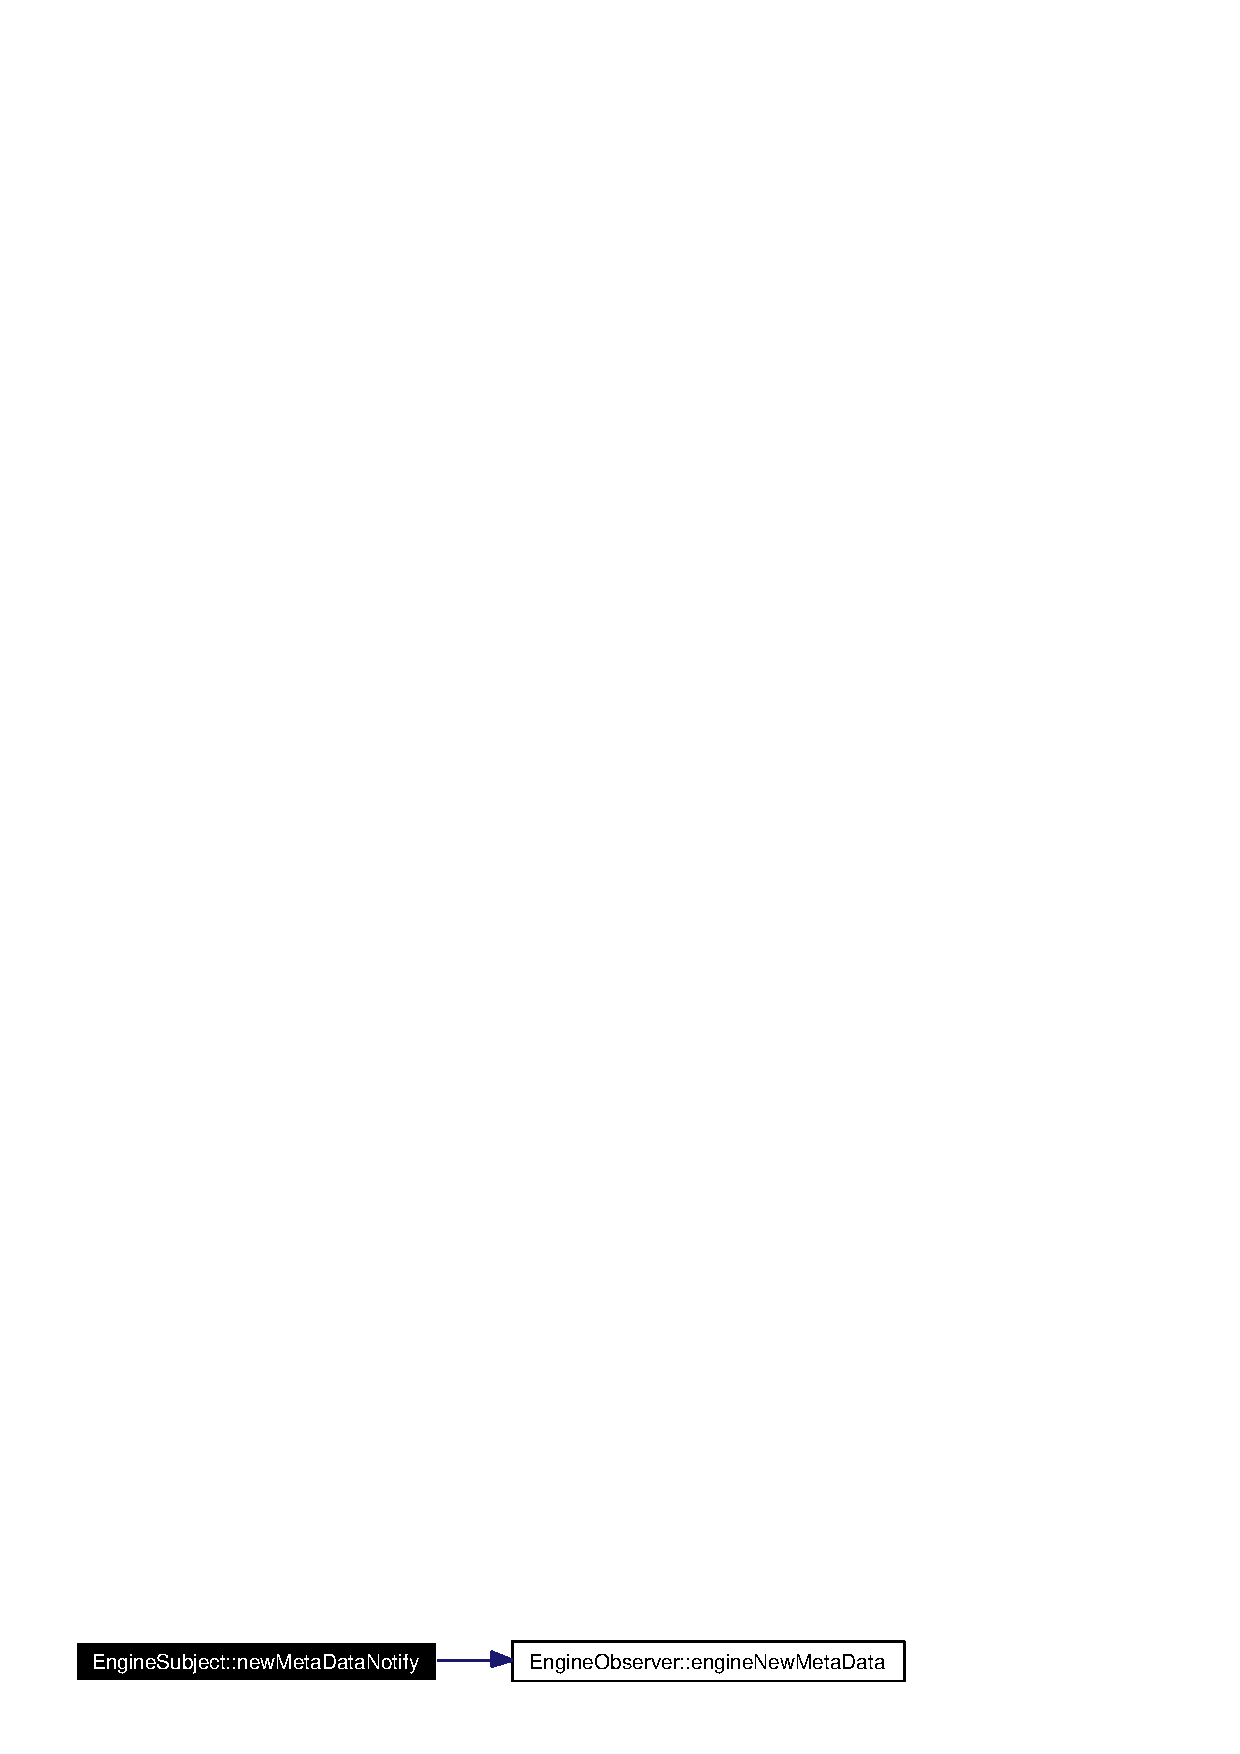
\includegraphics[width=217pt]{classEngineSubject_EngineSubjectb3_cgraph}
\end{center}
\end{figure}
\index{EngineSubject@{Engine\-Subject}!stateChangedNotify@{stateChangedNotify}}
\index{stateChangedNotify@{stateChangedNotify}!EngineSubject@{Engine\-Subject}}
\subsubsection{\setlength{\rightskip}{0pt plus 5cm}void Engine\-Subject::state\-Changed\-Notify ({\bf Engine\-Base::Engine\-State})\hspace{0.3cm}{\tt  [protected]}}\label{classEngineSubject_EngineSubjectb2}




Definition at line 44 of file engineobserver.cpp.

References Engine\-Observer::engine\-State\-Changed(), and Observers.

Referenced by Engine\-Controller::pause(), Engine\-Controller::play(), and Engine\-Controller::stop().



\footnotesize\begin{verbatim}45 {
46     QPtrListIterator<EngineObserver> it( Observers );
47     EngineObserver *observer;
48     while( ( observer = it.current() ) != 0 )
49     {
50         ++it;
51         observer->engineStateChanged( state );
52     }
53 }
\end{verbatim}\normalsize 


Here is the call graph for this function:\begin{figure}[H]
\begin{center}
\leavevmode
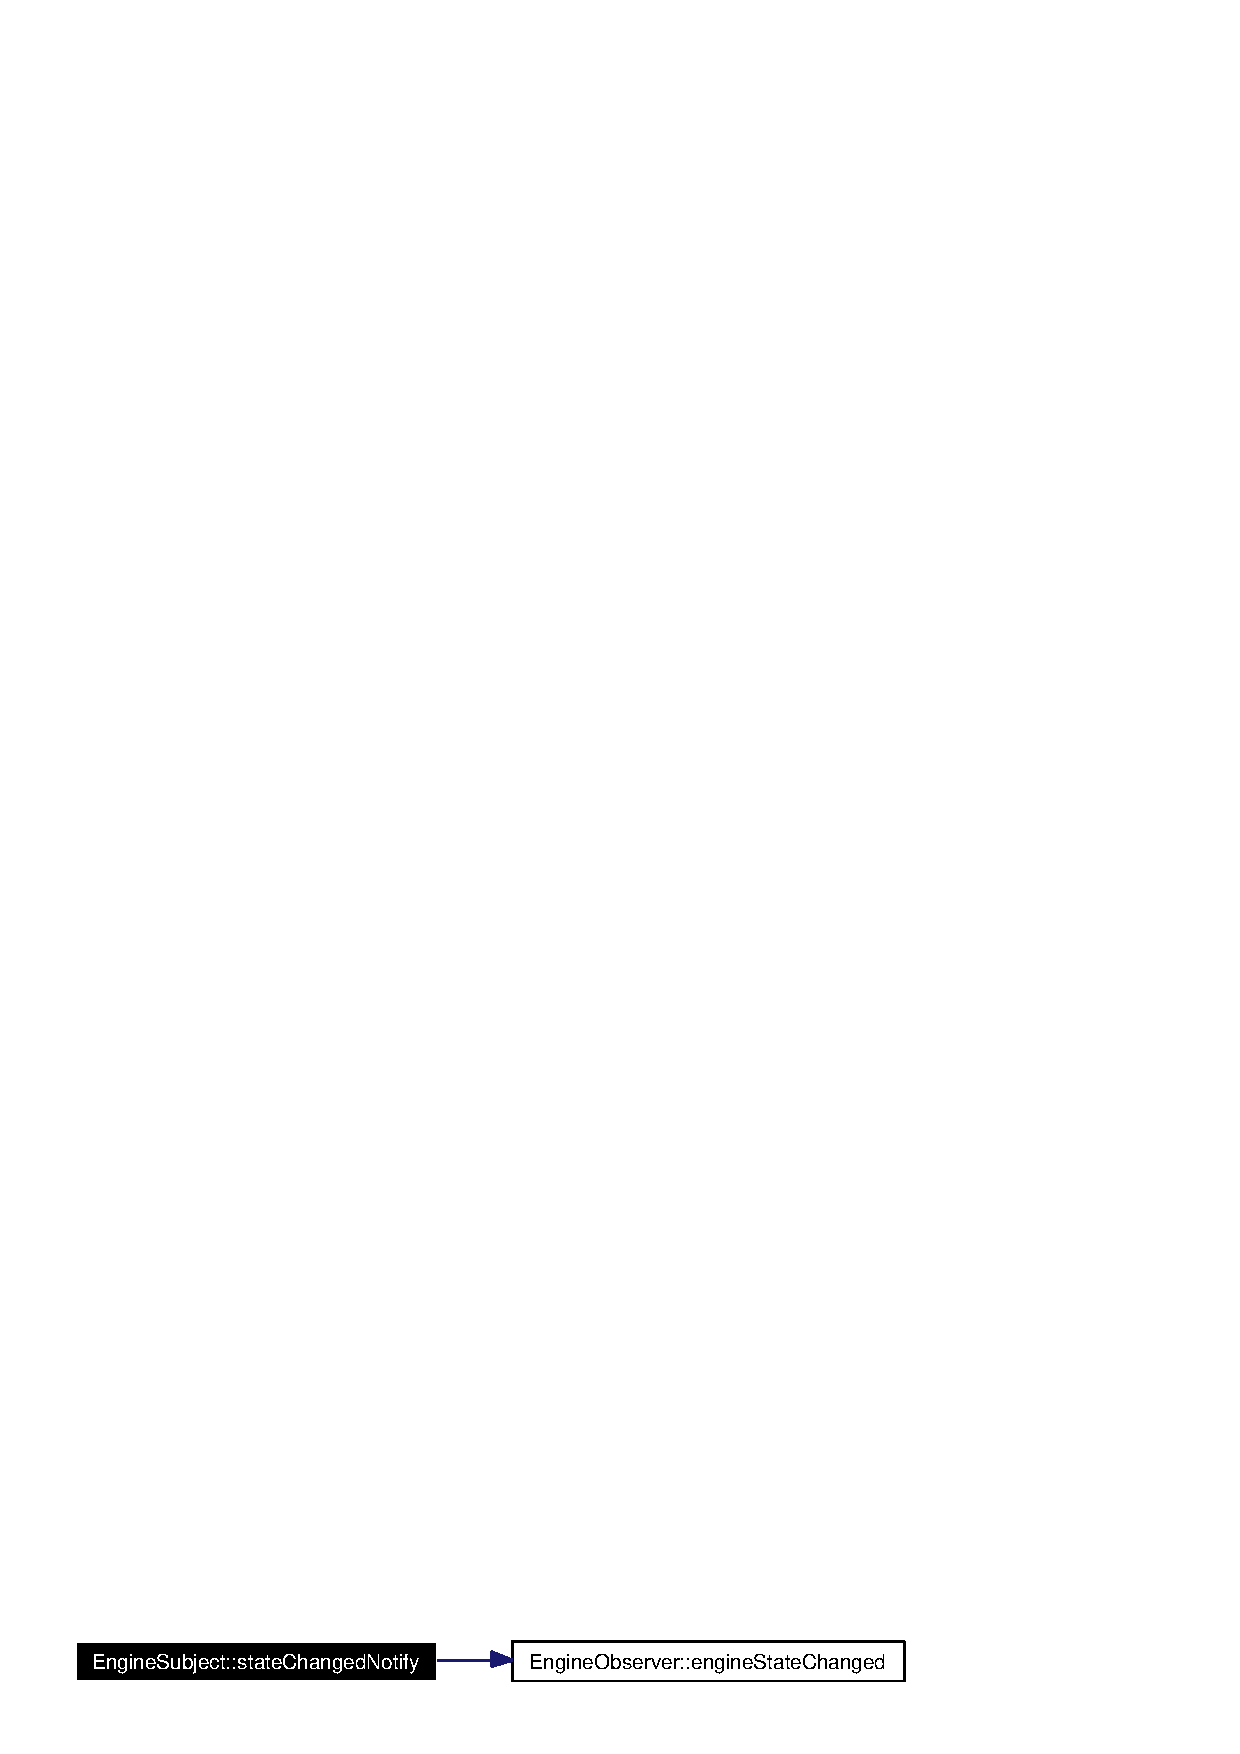
\includegraphics[width=217pt]{classEngineSubject_EngineSubjectb2_cgraph}
\end{center}
\end{figure}
\index{EngineSubject@{Engine\-Subject}!trackPositionChangedNotify@{trackPositionChangedNotify}}
\index{trackPositionChangedNotify@{trackPositionChangedNotify}!EngineSubject@{Engine\-Subject}}
\subsubsection{\setlength{\rightskip}{0pt plus 5cm}void Engine\-Subject::track\-Position\-Changed\-Notify (long)\hspace{0.3cm}{\tt  [protected]}}\label{classEngineSubject_EngineSubjectb5}




Definition at line 80 of file engineobserver.cpp.

References Engine\-Observer::engine\-Track\-Position\-Changed(), and Observers.

Referenced by Engine\-Controller::slot\-Main\-Timer().



\footnotesize\begin{verbatim}81 {
82     QPtrListIterator<EngineObserver> it( Observers );
83     EngineObserver *observer;
84     while( ( observer = it.current() ) != 0 )
85     {
86         ++it;
87         observer->engineTrackPositionChanged( position );
88     }
89 }
\end{verbatim}\normalsize 


Here is the call graph for this function:\begin{figure}[H]
\begin{center}
\leavevmode
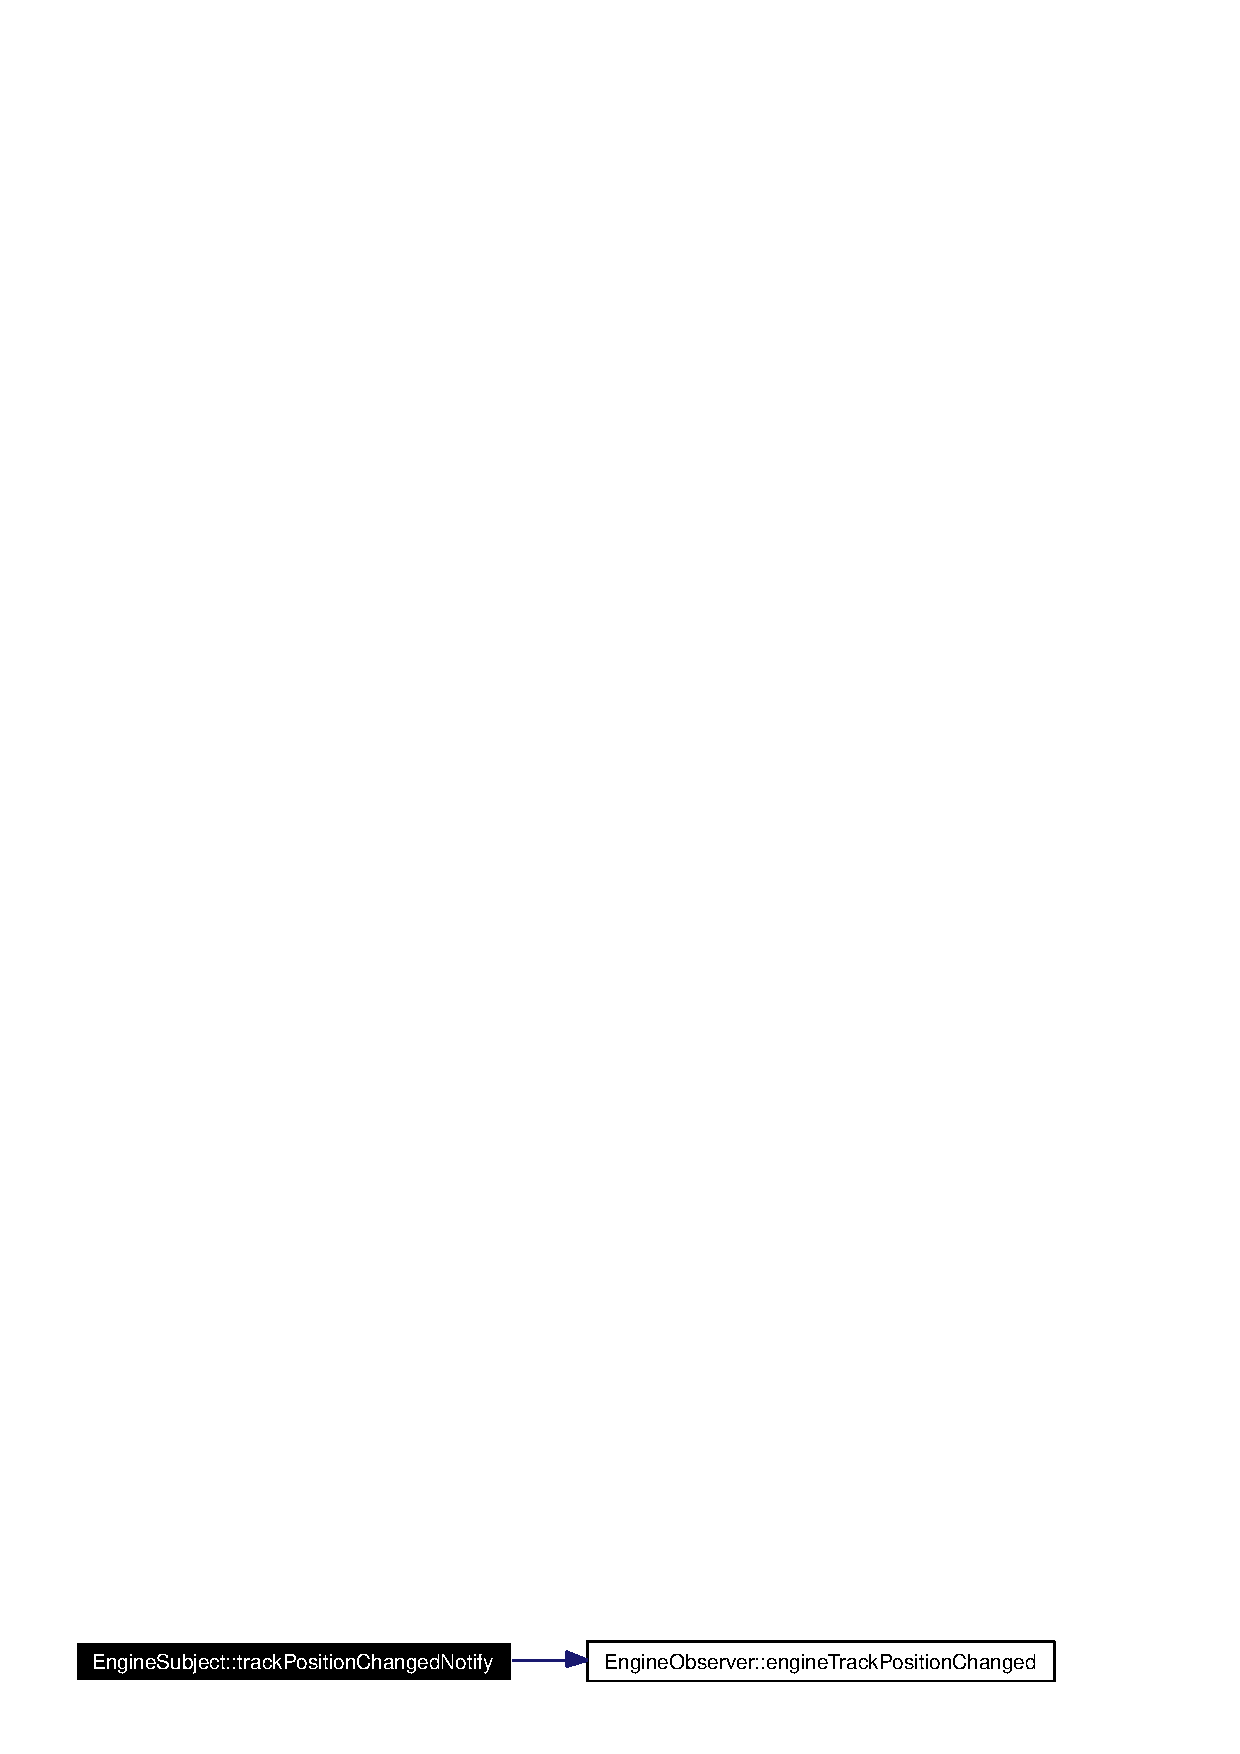
\includegraphics[width=253pt]{classEngineSubject_EngineSubjectb5_cgraph}
\end{center}
\end{figure}
\index{EngineSubject@{Engine\-Subject}!volumeChangedNotify@{volumeChangedNotify}}
\index{volumeChangedNotify@{volumeChangedNotify}!EngineSubject@{Engine\-Subject}}
\subsubsection{\setlength{\rightskip}{0pt plus 5cm}void Engine\-Subject::volume\-Changed\-Notify (int)\hspace{0.3cm}{\tt  [protected]}}\label{classEngineSubject_EngineSubjectb4}




Definition at line 68 of file engineobserver.cpp.

References Engine\-Observer::engine\-Volume\-Changed(), and Observers.

Referenced by Engine\-Controller::set\-Volume().



\footnotesize\begin{verbatim}69 {
70     QPtrListIterator<EngineObserver> it( Observers );
71     EngineObserver *observer;
72     while( ( observer = it.current() ) != 0 )
73     {
74         ++it;
75         observer->engineVolumeChanged( percent );
76     }
77 }
\end{verbatim}\normalsize 


Here is the call graph for this function:\begin{figure}[H]
\begin{center}
\leavevmode
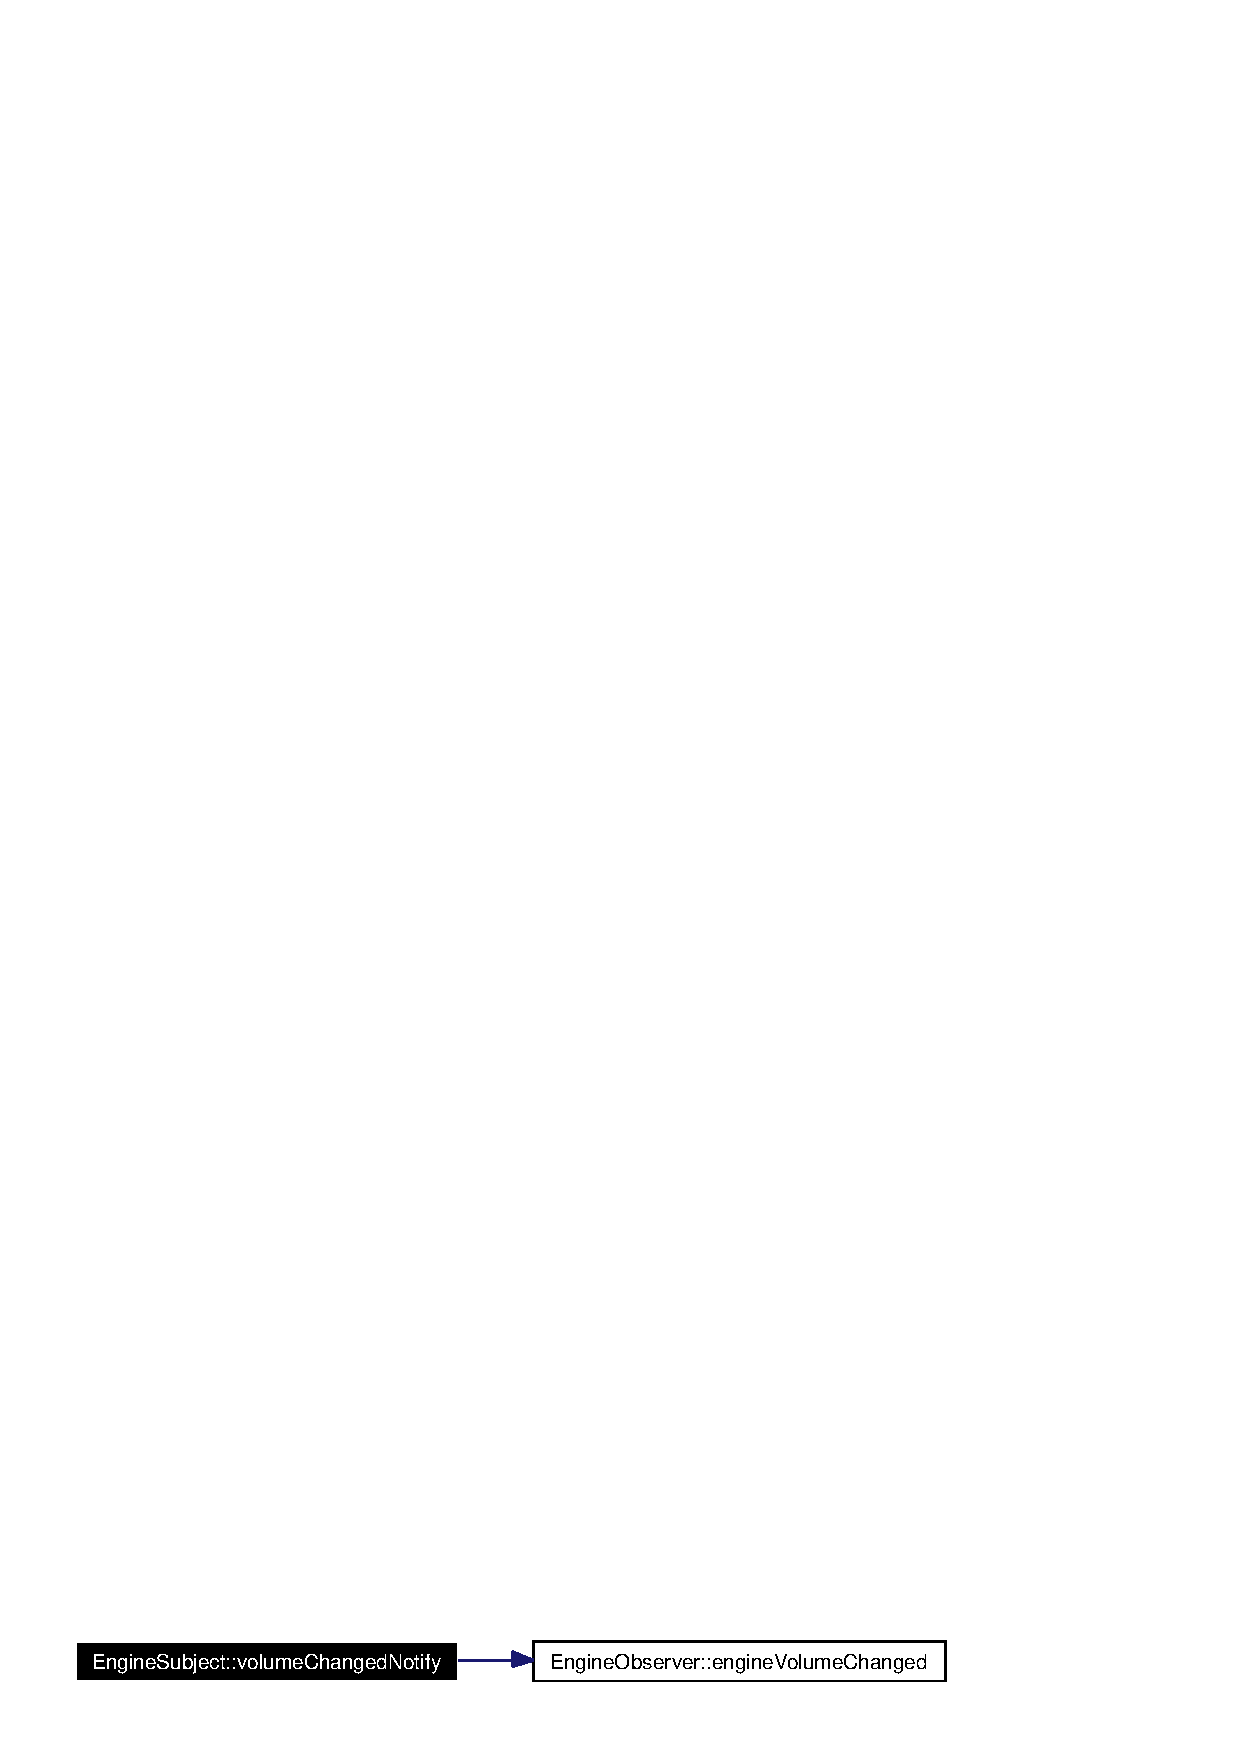
\includegraphics[width=227pt]{classEngineSubject_EngineSubjectb4_cgraph}
\end{center}
\end{figure}


\subsection{Member Data Documentation}
\index{EngineSubject@{Engine\-Subject}!Observers@{Observers}}
\index{Observers@{Observers}!EngineSubject@{Engine\-Subject}}
\subsubsection{\setlength{\rightskip}{0pt plus 5cm}QPtr\-List$<${\bf Engine\-Observer}$>$ {\bf Engine\-Subject::Observers}\hspace{0.3cm}{\tt  [private]}}\label{classEngineSubject_EngineSubjectr0}




Definition at line 60 of file engineobserver.h.

Referenced by attach(), detach(), new\-Meta\-Data\-Notify(), state\-Changed\-Notify(), track\-Position\-Changed\-Notify(), and volume\-Changed\-Notify().

The documentation for this class was generated from the following files:\begin{CompactItemize}
\item 
{\bf engineobserver.h}\item 
{\bf engineobserver.cpp}\end{CompactItemize}
